
\begin{frame}{Stijlen I}
	Bij bibliografie\"en is er een wildernis aan verschillende stijlen:
	
	\begin{itemize}
		\item \hll|numeric|: aa [2], bb [5, 6]\par
		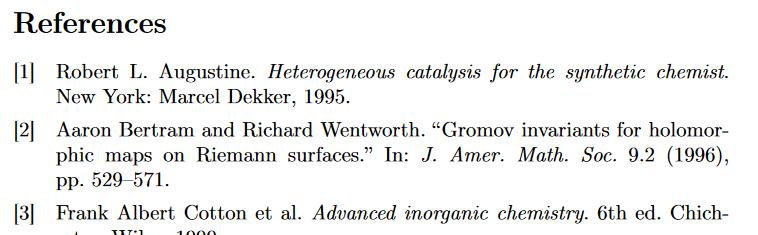
\includegraphics[width=0.8\textwidth]{assets/biblatexStyles/numericReferences.png}
		
		\item\hll|alphabetic|: aa [GMS94], bb [Gon01, Ham97]
		\item\hll|authoryear|: aa John 2003, bb ...
		\item\hll|apa|: aa (Lambert, 1993), bb ...
	\end{itemize}
	In APA: \hll|\\cite| en \hll|\\parencite| verschillen
\end{frame}

\updatehighlight{
	name=accentC,
	add={style=numeric}
}

\begin{saveblock}{codebox}
	%\highlightC{style=numeric}%
	\begin{highlightblock}
		\usepackage[style=numeric]{biblatex}
	\end{highlightblock}
\end{saveblock}

\updatehighlight{
	name=accentC,
	remove={style=numeric}
}

\begin{saveblock}{codeboxD}%
	\begin{highlightblock}
		\DeclareLanguageMapping{english}{english-apa}
	\end{highlightblock}
\end{saveblock}

\begin{frame}{Stijlen II}
	En er zijn nog veel meer stijlen! Voor exacte wetenschappen, gebruiken we gewoon numeric. Zo
	verander je de stijl:
	\useblock{codebox}
	
	\medskip
	Voor APA-stijl heb je daarnaast nodig:
	\useblock{codeboxD}
\end{frame}
